\documentclass[tikz,border=10pt]{standalone}
\usepackage{graphicx}

\begin{document}
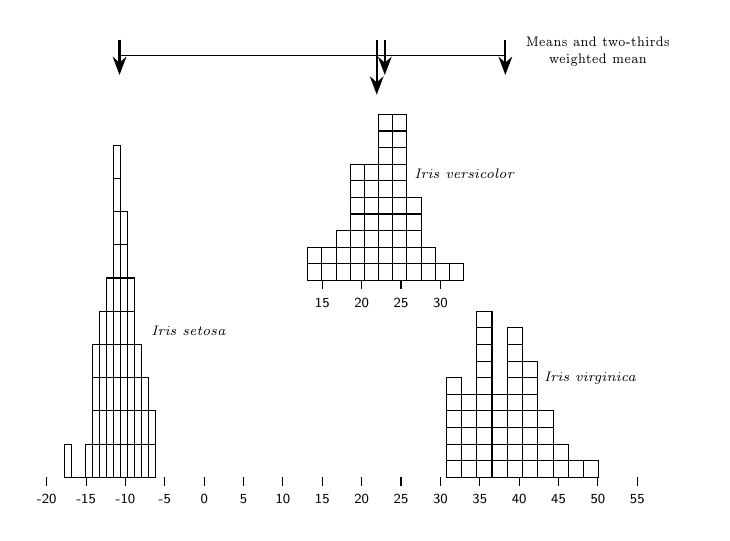
\begin{tikzpicture}[font=\sffamily\tiny]

\foreach \x in {-20,-15,...,55} {
  \draw (\x/10, 1pt) -- (\x/10, 4pt);
  \node at (\x/10, -4pt) {\x};
}

\def\xmin{-17.7109022}
\def\xmax{-6.2124275}
\def\n{13}
\pgfmathsetmacro{\w}{(\xmax-\xmin)/\n}
% высота одного блока
\def\cell{12pt}


\foreach \i/\v in {
1/1,2/0,3/0,4/1,5/4,6/5,7/6,8/10,9/8,10/6,11/4,12/3,13/2} 
{
  \pgfmathsetmacro{\xleft}{(\xmin + (\i-1)*\w)/10}
  \pgfmathsetmacro{\xright}{(\xmin + \i*\w)/10}
  \pgfmathsetmacro{\h}{\v*0.04}

% ======== особая обработка 2-го интервала ========
  \ifnum\i=2
     % пример: красный пустой столбик
  \draw[] (\xleft,10pt-6pt) rectangle (\xright,10pt-6pt);
  \else
  % ======== особая обработка 3-го интервала ========
     \ifnum\i=3
        % пример: заливка другим цветом
  \draw[] (\xleft,10pt-6pt) rectangle (\xright,10pt-6pt);
     \else
  % ======== обычная обработка всех остальных ========
  %\draw[] (\xleft,10pt) rectangle (\xright,10pt*\h*40);
  \draw[] (\xleft,10pt-6pt) rectangle (\xright, 10pt-6pt + \cell*\v);
  % разбиение на клетки
\foreach \k in {1,...,\v} {
  \draw (\xleft, 10pt-6pt + \cell*\k) -- (\xright, 10pt -6pt+ \cell*\k);
}
     \fi
  \fi

}


\def\xmina{30.7334647}
\def\xmaxa{50.1256323}
\def\na{10}
\pgfmathsetmacro{\wa}{(\xmaxa-\xmina)/\na}
% высота одного блока
\def\cella{6pt}


\foreach \i/\v in {
1/6,2/5,3/10,4/5,5/9,6/7,7/4,8/2,9/1,10/1} 
{
  \pgfmathsetmacro{\xleft}{(\xmina + (\i-1)*\wa)/10}
  \pgfmathsetmacro{\xright}{(\xmina + \i*\wa)/10}
  \pgfmathsetmacro{\ha}{\v*0.04}

  % ======== обычная обработка всех остальных ========
  \draw[] (\xleft,10pt-6pt) rectangle (\xright, 10pt -6pt+ \cella*\v);
  % разбиение на клетки
\foreach \k in {1,...,\v} {
  \draw (\xleft, 10pt -6pt+ \cella*\k) -- (\xright, 10pt -6pt+ \cella*\k);
}

}

\def\ttop{2.5cm}


\foreach \x in {15,20,...,30} {
  \draw (\x/10, \ttop+1pt) -- (\x/10, \ttop +   4pt);
  \node at (\x/10, \ttop -4pt) {\x};
}


\def\xminb{13.1562711	}
\def\xmaxb{32.94133}
\def\nb{11}
\pgfmathsetmacro{\wb}{(\xmaxb-\xminb)/\nb}
% высота одного блока
\def\cellb{6pt}


\foreach \i/\v in {
1/2,2/2,3/3,4/7,5/7,6/10,7/10,8/5,9/2,10/1,11/1} 
{
  \pgfmathsetmacro{\xleft}{(\xminb + (\i-1)*\wb)/10}
  \pgfmathsetmacro{\xright}{(\xminb + \i*\wb)/10}
  \pgfmathsetmacro{\hb}{\v*0.04}

  % ======== обычная обработка всех остальных ========
  \draw[] (\xleft,\ttop+10pt-6pt) rectangle (\xright,\ttop+ 10pt-6pt + \cellb*\v);
  % разбиение на клетки
\foreach \k in {1,...,\v} {
  \draw (\xleft, \ttop+10pt -6pt+ \cellb*\k) -- (\xright, \ttop+10pt-6pt + \cellb*\k);
}

}


\draw (-10.75042/10, 5.5cm) -- (38.24827/10, 5.5cm);

\usetikzlibrary {arrows.meta}

\draw [thick,arrows = {-Stealth}] (-10.75042/10, 5.7cm) -> (-10.75042/10, 5.25cm);
\draw [thick,arrows = {-Stealth}] (22.93888/10, 5.7cm) -> (22.93888/10, 5.25cm);
\draw [thick,arrows = {-Stealth}] (38.24827/10, 5.7cm) -> (38.24827/10, 5.25cm);

% Это просто точка, расположенная на \( \tfrac{2}{3} \) пути от среднего \emph{setosa} к среднему \emph{virginica}.
% Формула и эквивалентные формы:
% \[
% m = \mu_{\text{setosa}} + \tfrac{2}{3}(\mu_{\text{virginica}}-\mu_{\text{setosa}})
% \]
% что равно
% \[
% m = \tfrac{1}{3}\mu_{\text{setosa}} + \tfrac{2}{3}\mu_{\text{virginica}}.
% \]
% 
% Подставим числа:
% \[
% m = -10.75042 + \tfrac{2}{3}(38.24827 - (-10.75042)) = 21.91537\ (\approx 21.92).
% \]
\draw [thick,arrows = {-Stealth}] (21.91537/10, 5.7cm) -- (21.91537/10, 5.0cm);


\node[font=\itshape\tiny] at (-0.2cm, 2cm) {Iris setosa};
\node[font=\itshape\tiny] at (3.3cm, 4cm) {Iris versicolor};
\node[font=\itshape\tiny] at (4.9cm, 1.4cm) {Iris virginica};


\node[font=\tiny]  at (5.0cm,5.55cm) {\scalebox{0.8}[1]{\parbox{3cm}{\centering\tiny
Means and two-thirds\\
weighted mean}}};

\end{tikzpicture}
\end{document}